\documentclass{article}
\usepackage[a4paper]{geometry}
\usepackage[T1]{fontenc}
\usepackage[utf8]{inputenc}
\usepackage[italian]{babel}
\usepackage{geometry}
\usepackage[font={small,sl}]{caption}
\usepackage[section]{placeins}
\usepackage{graphicx}
\usepackage[table, dvipsnames]{xcolor}
\usepackage{subcaption}
\usepackage{listings}
\usepackage{fancyhdr}
\usepackage{amssymb}
\usepackage{amsmath}
\usepackage[font={small,sl}]{caption}
\usepackage{hyperref}

\def\code#1{\texttt{#1}}

\setlength{\parskip}{1em}
\setlength{\parindent}{0em}
\setlength{\arrayrulewidth}{0.1em}

\hypersetup{
    colorlinks=true,
    citecolor=blue,
    linkcolor=blue,
    linktocpage=true,
    urlcolor=blue,
    pdftitle={Relazione Progetto SOA},
    pdfauthor={C. Cuffaro}
}

% Colori per i listing
\definecolor{code_red}{rgb}{0.6,0,0} % strings
\definecolor{code_green}{rgb}{0.25,0.5,0.35} % comments
\definecolor{code_purple}{rgb}{0.5,0,0.35} % keywords
\definecolor{code_background}{rgb}{0.95,0.95,0.92} % background

% Stile del codice standard (C)
\lstset{
	language=C, 
	backgroundcolor=\color{code_background},
	frame=single,
	basicstyle=\ttfamily\small,
	keywordstyle=\color{code_purple}\bfseries\small,
	stringstyle=\color{code_red}\small,
	commentstyle=\color{code_green}\small,
	numbers=left,
	numberstyle=\small\color{gray},
	numbersep=5pt,
	tabsize=4,
	showtabs=false,
	showspaces=false,
	showstringspaces=false,
	escapechar=|, 
	captionpos=b,
	breaklines=true,
}

\renewcommand{\lstlistingname}{Snippet}

\pagestyle{fancy}
\fancyhf{}
\lhead{\small C. Cuffaro}
\rhead{\small Relazione Progetto SOA}
\cfoot{\thepage}
%\cfoot{Pagina \thepage}

\begin{document}
\author{%
Cristiano Cuffaro \\
{\small matricola: \texttt{0299838}} \\
{\small \texttt{cristiano.cuffaro@outlook.com}}
}
\title{Relazione Progetto SOA}
\date{A.A. 2021-2022}

\maketitle
\tableofcontents
\newpage

\section{Rappresentazione dei device file}
In accordo alla specifica del progetto e ai casi d'uso che si possono derivare da essa, è stata scelta una rappresentazione in RAM per i \textsl{multi-flow device file}.

In particolare, uno stream di dati è implementato come una \textsl{linked list} di segmenti di dati dinamicamente allocati e agganciati tra una \textsl{head} ed una \textsl{tail} fittizie, come mostrato nella rappresentazione in figura \ref{fig-1}.

\captionsetup[figure]{justification=centering}
\begin{figure}[ht]
\centering
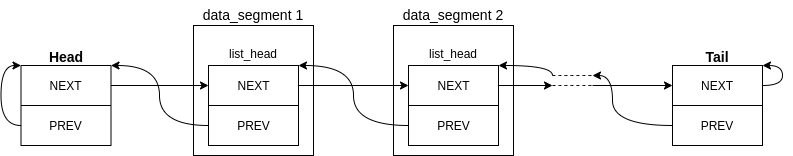
\includegraphics[width=0.8\textwidth]{img/segment-list}
\caption{Lista di segmenti che implementa un data stream}
\label{fig-1}
\end{figure}

Per ciascun segmento di dati, all'interno di una struttura \texttt{data\_segment} sono mantenute le seguenti informazioni:
\begin{itemize}
\item un puntatore ai dati effettivi;
\item la dimensione corrente dei dati;
\item un indice che rappresenta la posizione corrente di lettura;
\item una struttura \texttt{list\_head} per il collegamento alla lista.
\end{itemize}
Quando è necessario allocare un nuovo segmento di dati, avviene un'unica chiamata verso lo \textsl{SLAB allocator} per ottenere un'area di memoria in cui impaccare la struttura dati nella parte alta e i dati effettivi in quella bassa. Inoltre, per limitare la dimensione reale della struttura a 40 byte è stata definita specificando l'attributo \texttt{packed}.

In una struttura \texttt{device\_struct} sono definite le informazioni associate a ciascun device, in particolare:
\begin{itemize}
\item una waitqueue per ciascun data stream, ove si tiene traccia dei thread in attesa di prelevare o scaricare dati nel caso di letture o scritture bloccanti;
\item una workqueue per mantenere il lavoro da eseguire in maniera \textsl{delayed} nel caso di scritture a bassa priorità;
\item un mutex per ciascun data stream, necessario per sincronizzare le operazioni di lettura e scrittura;
\item una struttura \texttt{segment\_list} per ciascun data stream, contenente gli elementi fittizi della lista;
\item il numero di byte validi in ciascun data stream, ovvero quelli effettivamente leggibili;
\item il numero di byte liberi in ciascun data stream, ovvero quelli che determinano la possibilità di eseguire delle operazioni di scrittura;
\item il numero di thread in attesa di dati per ciascun data stream, ovvero la cardinalità dell'insieme dei lettori all'interno della corrispondente waitqueue.
\end{itemize}
Per aumentare il livello di sicurezza del VFS, per questa struttura dati è stata utilizzata la dicitura \texttt{\_\_randomize\_layout}, in modo tale che un eventuale attacco finalizzato a prelevare informazioni da un device file sia ostacolato dal fatto che lo spiazzamento a cui sono presenti i dati è arbitrario e cambia tra i vari kernel.

\section{Operazioni sui multi-flow device file}
Nelle seguenti sottosezioni sono descritte le funzioni che costituiscono il driver, ovvero che permettono di eseguire le varie operazioni sui device file che esso gestisce.

\subsection{Operazione di apertura}
La funzione \texttt{mfd\_open} consente l'apertura di un multi-flow device file. Ad ogni invocazione, la funzione verifica che il minor number associato al dispositivo sia gestibile dal driver e che esso non sia correntemente disabilitato. Se i controlli vanno a buon fine, viene allocata la memoria per ospitare una struttura \texttt{session\_data} contenente le seguenti informazioni:
\begin{itemize}
\item il livello di priorità dello stream di dati su cui si sta correntemente lavorando (bassa priorità per default);
\item l'intervallo di tempo che determina la massima attesa per le operazioni di lettura e scrittura bloccanti (10 secondi per default).
\end{itemize}
Per mantenere il puntatore a questa struttura viene sfruttato il campo \texttt{.private\_data} della struttura \texttt{file} corrispondente alla sessione di I/O.

Per determinare se l'operazione di apertura è stata eseguita in modalità non bloccante, viene controllato se all'interno del campo \texttt{file->f\_flags} è settato il flag \texttt{O\_NONBLOCK}. In caso di operazioni non bloccanti, tutte le allocazioni di memoria vengono eseguite specificando la maschera \texttt{GFP\_ATOMIC}, grazie alla quale la chiamata verso l'allocatore di memoria può fallire senza portare il thread a dormire qualora non vi fosse memoria immediatamente disponibile.

\subsection{Operazione di rilascio}
La funzione \texttt{mfd\_release} è invocata quando viene rilasciata la struttura \texttt{file} e, in maniera duale rispetto alla \texttt{mfd\_open}, si occupa di riconsegnare all'allocatore l'area di memoria puntata da \texttt{file->private\_data}.

\subsection{Operazione di lettura}
La funzione \texttt{mfd\_read} viene invocata quando si esegue un'operazione di lettura su un multi-flow device file.

Se per la sessione di I/O è settato il flag \texttt{O\_NONBLOCK}, viene fatto quanto segue:
\begin{enumerate}
\item si esegue una trylock sul mutex relativo allo stream di dati da cui si vuole leggere;
\item si verifica se la quantità di dati leggibili è pari a zero;
\end{enumerate}
se fallisce l'acquisizione del mutex o non ci sono dati da leggere, la funzione restituisce \texttt{-EAGAIN}.

Se l'operazione di lettura è eseguita in modalità bloccante, si procede come segue:
\begin{enumerate}
\item viene incrementato il numero di thread in attesa di dati provenienti dal data stream in questione;
\item viene invocata l'API \texttt{wait\_event\_interruptible\_timeout} specificando:
\begin{enumerate}
\item la waitqueue corrispondente al data stream;
\item la condizione che determina il risveglio dei thread;
\item il timeout specificato nei dati di sessione;
\end{enumerate}
\item se il thread esce dal sonno per via del termine del timeout o per una segnalazione, la funzione restituisce l'errore corrispondente.
\end{enumerate}
Per far sì che ogni \textsl{wake up} porti al risveglio di al più un thread posto sulla waitqueue, invece di specificare direttamente alla wait event API la condizione che il numero di byte leggibili sia maggiore di zero, viene specificata la macro \texttt{lock\_and\_check}, mostrata nello snippet \ref{lst-1}.
\begin{lstlisting}[label=lst-1, caption={Macro \texttt{lock\_and\_check}}]
#define lock_and_check(condition, mutexp)       \
({                                              \
        int __ret = 0;                          \
        if (mutex_trylock(mutexp)) {            \
                if (condition)                  \
                        __ret = 1;              \
                else                            \
                        mutex_unlock(mutexp);   \
        }                                       \
        __ret;                                  \
})
\end{lstlisting}
Grazie ad essa, è possibile provare ad acquisire il lock prima di controllare la condizione reale su cui eventualmente dormire; per cui un solo thread ha la possibilità di risvegliarsi avendo già acquisito il lock, se la condizione è soddisfatta. In tutti gli altri casi si rimane in sleep.

Una volta usciti dalla wait event API, si decrementa il numero di thread in attesa e si prosegue con la lettura effettiva dei dati.

Sia nel caso di operazione bloccante che non, la lettura effettiva è realizzata invocando la funzione \texttt{actual\_read} ...

\end{document}